% Options for packages loaded elsewhere
\PassOptionsToPackage{unicode}{hyperref}
\PassOptionsToPackage{hyphens}{url}
%
\documentclass[
]{article}
\title{Predictive performance of multi-model ensemble forecasts of
COVID-19 across European nations}
\author{}
\date{\vspace{-2.5em}}

\usepackage{amsmath,amssymb}
\usepackage{lmodern}
\usepackage{iftex}
\ifPDFTeX
  \usepackage[T1]{fontenc}
  \usepackage[utf8]{inputenc}
  \usepackage{textcomp} % provide euro and other symbols
\else % if luatex or xetex
  \usepackage{unicode-math}
  \defaultfontfeatures{Scale=MatchLowercase}
  \defaultfontfeatures[\rmfamily]{Ligatures=TeX,Scale=1}
\fi
% Use upquote if available, for straight quotes in verbatim environments
\IfFileExists{upquote.sty}{\usepackage{upquote}}{}
\IfFileExists{microtype.sty}{% use microtype if available
  \usepackage[]{microtype}
  \UseMicrotypeSet[protrusion]{basicmath} % disable protrusion for tt fonts
}{}
\makeatletter
\@ifundefined{KOMAClassName}{% if non-KOMA class
  \IfFileExists{parskip.sty}{%
    \usepackage{parskip}
  }{% else
    \setlength{\parindent}{0pt}
    \setlength{\parskip}{6pt plus 2pt minus 1pt}}
}{% if KOMA class
  \KOMAoptions{parskip=half}}
\makeatother
\usepackage{xcolor}
\IfFileExists{xurl.sty}{\usepackage{xurl}}{} % add URL line breaks if available
\IfFileExists{bookmark.sty}{\usepackage{bookmark}}{\usepackage{hyperref}}
\hypersetup{
  pdftitle={Predictive performance of multi-model ensemble forecasts of COVID-19 across European nations},
  hidelinks,
  pdfcreator={LaTeX via pandoc}}
\urlstyle{same} % disable monospaced font for URLs
\usepackage[margin=1in]{geometry}
\usepackage{graphicx}
\makeatletter
\def\maxwidth{\ifdim\Gin@nat@width>\linewidth\linewidth\else\Gin@nat@width\fi}
\def\maxheight{\ifdim\Gin@nat@height>\textheight\textheight\else\Gin@nat@height\fi}
\makeatother
% Scale images if necessary, so that they will not overflow the page
% margins by default, and it is still possible to overwrite the defaults
% using explicit options in \includegraphics[width, height, ...]{}
\setkeys{Gin}{width=\maxwidth,height=\maxheight,keepaspectratio}
% Set default figure placement to htbp
\makeatletter
\def\fps@figure{htbp}
\makeatother
\setlength{\emergencystretch}{3em} % prevent overfull lines
\providecommand{\tightlist}{%
  \setlength{\itemsep}{0pt}\setlength{\parskip}{0pt}}
\setcounter{secnumdepth}{-\maxdimen} % remove section numbering
\newlength{\cslhangindent}
\setlength{\cslhangindent}{1.5em}
\newlength{\csllabelwidth}
\setlength{\csllabelwidth}{3em}
\newlength{\cslentryspacingunit} % times entry-spacing
\setlength{\cslentryspacingunit}{\parskip}
\newenvironment{CSLReferences}[2] % #1 hanging-ident, #2 entry spacing
 {% don't indent paragraphs
  \setlength{\parindent}{0pt}
  % turn on hanging indent if param 1 is 1
  \ifodd #1
  \let\oldpar\par
  \def\par{\hangindent=\cslhangindent\oldpar}
  \fi
  % set entry spacing
  \setlength{\parskip}{#2\cslentryspacingunit}
 }%
 {}
\usepackage{calc}
\newcommand{\CSLBlock}[1]{#1\hfill\break}
\newcommand{\CSLLeftMargin}[1]{\parbox[t]{\csllabelwidth}{#1}}
\newcommand{\CSLRightInline}[1]{\parbox[t]{\linewidth - \csllabelwidth}{#1}\break}
\newcommand{\CSLIndent}[1]{\hspace{\cslhangindent}#1}
\usepackage{booktabs}
\usepackage{longtable}
\usepackage{array}
\usepackage{multirow}
\usepackage{wrapfig}
\usepackage{float}
\usepackage{colortbl}
\usepackage{pdflscape}
\usepackage{tabu}
\usepackage{threeparttable}
\usepackage{threeparttablex}
\usepackage[normalem]{ulem}
\usepackage{makecell}
\usepackage{xcolor}
\ifLuaTeX
  \usepackage{selnolig}  % disable illegal ligatures
\fi

\begin{document}
\maketitle

\emph{Order tbc;} Katharine Sherratt, Hugo Gruson, \emph{Any
co-authors}, \emph{Team authors}, \emph{Advisory team authors},
\emph{ECDC authors}, Johannes Bracher, Sebastian Funk

\emph{(Acknowledge first round contributions: Bastian Prasse, Enrique
Alvarez-Lacalle, Sam Abbott; also: Marco Mingione, Francesco Bartolucci,
Jan Meinke, Jan Pablo Burgard, Stefan Heyder, Veronika Eclerová, Clara
Prats Soler, Aniruddha Adiga, Fulvia Pennoni)}

\hypertarget{abstract}{%
\section{Abstract}\label{abstract}}

\emph{Background} Short-term forecasts of infectious disease burden can
contribute to situational awareness and aid capacity planning. Based on
best practice in other fields and recent insights in infectious disease
epidemiology, one can maximise the predictive performance of such
forecasts if multiple models are combined into an ensemble. Here we
report on the performance of ensembles in predicting COVID-19 cases and
deaths across Europe between 08 March 2021 and 07 March 2022.

\emph{Methods} We used open-source tools to develop a public European
COVID-19 Forecast Hub. We invited groups globally to contribute weekly
forecasts for COVID-19 cases and deaths over the next one to four weeks.
Forecasts were submitted using standardised quantiles of the predictive
distribution. Each week we created an ensemble forecast, where each
predictive quantile was calculated as the equally-weighted average
(initially the mean and then the median from the 26th of July) of all
individual models' predictive quantiles. We measured the performance of
each model using the relative Weighted Interval Score (WIS), comparing
models' forecast accuracy relative to all other models, then scaled
against a baseline model of no change. We retrospectively explored
alternative methods for ensemble forecasts, including weighted averages
based on models' past predictive performance.

\emph{Results} Over 52 weeks we collected and combined up to 28 forecast
models for 32 countries. We found a weekly ensemble had a strong and
consistently reliable performance across countries over time. Across all
horizons and locations, the ensemble performed better on scaled relative
WIS than 84\% of participating models' forecasts of incident cases (with
a total N=862), and 92\% of participating models' forecasts of deaths
(N=746). Across a one to four week time horizon, ensemble performance
declined with longer forecast periods when forecasting cases, but
remained stable over four weeks for incident death forecasts. In every
forecast across 32 countries, the ensemble outperformed 50\% of
submitted models when forecasting either cases or deaths, frequently
outperforming all of its individual component models. Among several
choices of ensemble methods we found that the most influential and best
choice was to use a median average of models instead of using the mean,
regardless of methods of weighting component forecast models.

\emph{Conclusions} Our results support the use of combining forecasts
from individual models into an ensemble in order to improve predictive
performance across epidemiological targets and populations during
infectious disease epidemics. Our findings suggested that for an
emerging pathogen with many individual models, median ensemble methods
may improve predictive performance more than mean ensemble methods. Our
findings also highlight that forecast consumers should place more weight
on incident death forecasts versus incident case forecasts for forecast
horizons greater than two weeks.

\emph{Code and data availability} All data and code are publicly
available on Github: covid19-forecast-hub-europe/euro-hub-ensemble.

\emph{This document was generated on} 2022-03-30

\hypertarget{background}{%
\section{Background}\label{background}}

Epidemiological forecasts make quantitative statements about a disease
outcome in the near future. Forecasting targets can include measures of
prevalent or incident disease and its severity, for some population over
a specified time horizon. Researchers, policy makers, and the general
public have used such forecasts to understand and respond to the global
outbreaks of COVID-19 since early 2020
\protect\hyperlink{ref-basshuysenThreeWaysWhich2021}{{[}1{]}}.
Forecasters use a variety of methods and models for creating and
publishing forecasts, varying in both defining the forecast outcome and
in reporting the probability distribution of outcomes
\protect\hyperlink{ref-zelnerAccountingUncertaintyPandemic2021}{{[}2{]}},
\protect\hyperlink{ref-jamesUseMisuseMathematical2021}{{[}3{]}}. Such
variation between forecasts makes it difficult to compare predictive
performance between forecast models. These barriers to comparing and
evaluating forecasts make it difficult to derive objective arguments for
using one forecast over another. This hampers the selection of a
representative forecast and hinders finding a reliable basis for
decisions.

A ``forecast hub'' is a centralised effort to improve the transparency
and usefulness of forecasts, by standardising and collating the work of
many independent teams producing forecasts
\protect\hyperlink{ref-reichCollaborativeMultiyearMultimodel2019}{{[}4{]}}.
A hub sets a commonly agreed-upon structure for forecast targets, such
as type of disease event, spatio-temporal units, or the set of quantiles
of the probability distribution to include from probabilistic forecasts.
For instance, a hub may collect predictions of the total number of cases
reported in a given country for each day in the next two weeks.
Forecasters can adopt this format and contribute forecasts for
centralised storage in the public domain. This shared infrastructure
allows forecasts produced from diverse teams and methods to be
visualised and quantitatively compared on a like-for-like basis, which
can strengthen public and policy use of disease forecasts
\protect\hyperlink{ref-cdcCoronavirusDisease20192020}{{[}5{]}}. The
underlying approach to creating a forecast hub was pioneered for
forecasting influenza in the USA and adapted for forecasts of short-term
COVID-19 cases and deaths in the US
\protect\hyperlink{ref-cramerUnitedStatesCOVID192021}{{[}6{]}},
\protect\hyperlink{ref-rayEnsembleForecastsCoronavirus2020e}{{[}7{]}},
with similar efforts elsewhere
\protect\hyperlink{ref-bracherPreregisteredShorttermForecasting2021}{{[}8{]}}--\protect\hyperlink{ref-bicherSupportingCOVID19PolicyMaking2021}{{[}10{]}}.

Standardising forecasts allows for combining multiple forecasts into a
single ensemble with the potential for an improved predictive
performance. Evidence from previous efforts in multi-model infectious
disease forecasting suggests that forecasts from an ensemble of models
can be consistently high performing compared to any one of the component
models
\protect\hyperlink{ref-reichAccuracyRealtimeMultimodel2019}{{[}11{]}}--\protect\hyperlink{ref-viboudRAPIDDEbolaForecasting2018}{{[}13{]}}.
Elsewhere, weather forecasting has a long-standing use of building
ensembles of models using diverse methods with standardised data and
formatting in order to improve performance
\protect\hyperlink{ref-buizzaIntroductionSpecialIssue2019}{{[}14{]}},
\protect\hyperlink{ref-moranEpidemicForecastingMessier2016}{{[}15{]}}.

The European COVID-19 Forecast Hub
\protect\hyperlink{ref-europeancovid-19forecasthubEuropeanCOVID19Forecast2021}{{[}16{]}}
is a project to collate short term forecasts of COVID-19 across 32
countries in the European region. The Hub is funded and supported by the
European Centre for Disease Prevention and Control (ECDC), with the
primary aim to provide reliable information about the near-term
epidemiology of the COVID-19 pandemic to the research and policy
communities and the general public. Second, the Hub aims to create
infrastructure for storing and analysing epidemiological forecasts made
in real time by diverse research teams and methods across Europe. Third,
the Hub aims to maintain a community of infectious disease modellers
underpinned by open science principles.

We started formally collating and combining contributions to the
European Forecast Hub in March 2021. Here, we investigate the predictive
performance of an ensemble of all forecasts contributed to the Hub in
real time each week, as well as the performance of variations of
ensemble methods created retrospectively.

\hypertarget{methods}{%
\section{Methods}\label{methods}}

We developed infrastructure to host and analyse forecasts, focussing on
compatibility with the US
\protect\hyperlink{ref-cramerReichlabCovid19forecasthubRelease2021}{{[}17{]}},
\protect\hyperlink{ref-wangReichlabCovidHubUtilsRepository2021}{{[}18{]}}
and the German and Polish COVID-19
\protect\hyperlink{ref-bracherGermanPolishCOVID192020}{{[}19{]}}
forecast hubs.

\hypertarget{forecast-targets-and-standardisation}{%
\subsubsection{Forecast targets and
standardisation}\label{forecast-targets-and-standardisation}}

We sought forecasts for two measures of COVID-19 incidence: the total
reported number of cases and deaths per week. We considered forecasts
for 32 countries in Europe, including all countries of the European
Union and European Free Trade Area, and the United Kingdom. We compared
forecasts against observed data reported by Johns Hopkins University
(JHU,
\protect\hyperlink{ref-dongInteractiveWebbasedDashboard2020}{{[}20{]}}).
JHU data included a mix of national and aggregated subnational data for
the 32 countries in the Hub. Incidence was aggregated over the Morbidity
and Mortality Weekly Report (MMWR) epidemiological week definition of
Sunday through Saturday.

When predicting any single forecast target, teams could express
uncertainty by submitting predictions across a range of a pre-specified
set of 23 quantiles in the probability distribution. Teams could also
submit a single point forecast without uncertainty. At the first
submission we asked teams to add a single set of metadata briefly
describing the forecasting team and methods. No restrictions were placed
on who could submit forecasts, and to increase participation we actively
contacted known forecasting teams across Europe and the US and
advertised among the ECDC network. Teams submitted a broad spectrum of
model types, ranging from mechanistic to empirical models, agent-based
and statistical models, and ensembles of multiple quantitative or
qualitative models (described at
\url{https://covid19forecasthub.eu/community.html}). We maintain a full
project specification with a detailed submissions protocol
\protect\hyperlink{ref-europeancovid-19forecasthubCovid19forecasthubeuropeWiki}{{[}21{]}}.

With the complete dataset for the latest forecasting week available each
Sunday, teams typically submitted forecasts to the hub on Monday. We
implemented an automated validation programme to check that each new
forecast conformed to standardised formatting. The validation step
ensured a monotonic increase of predictions with each increasing
quantile, integer-valued counts of predicted cases, as well as
consistent date and location definitions.

Each week we built an ensemble of all forecasts updated after all
forecasts had been validated. From the first week of forecasting from 8
March 2021, the ensemble method for summarising across forecasts was the
arithmetic mean of all models at each predictive quantile for a given
location, target, and horizon. From 26 July 2021 onwards the ensemble
instead used a median of all predictive quantiles, in order to mitigate
the wide uncertainty produced by some highly anomalous forecasts. We
created an open and publicly accessible interface to the forecasts and
ensemble, including an online visualisation tool allowing viewers to see
past data and interact with one or multiple forecasts for each country
and target for up to four weeks' horizon
\protect\hyperlink{ref-europeancovid-19forecasthubEuropeanCovid19Forecast}{{[}22{]}}.
All forecast and meta data are freely available and held on Zoltar, a
platform for hosting epidemiological forecasts
\protect\hyperlink{ref-epiforecastsProjectECDCEuropean2021}{{[}23{]}},
\protect\hyperlink{ref-reichZoltarForecastArchive2021}{{[}24{]}}.

\hypertarget{forecast-evaluation}{%
\subsubsection{Forecast evaluation}\label{forecast-evaluation}}

We evaluated all previous forecasts against actual observed values for
each model, stratified by the forecast horizon, location, and target. We
calculated scores using the scoringutils R package
\protect\hyperlink{ref-nikosibosseScoringutilsUtilitiesScoring2020}{{[}25{]}}.
We removed any forecast surrounding (in the week of the first week
after) a strongly anomalous data point. We defined anomalous as where
any subsequent data release revised that data point by over 5\%.

For each model, we established its overall predictive performance using
the weighted interval score (WIS) and the accuracy of its prediction
boundaries as the coverage of the predictive intervals. We calculated
coverage at a given interval level k, where \(k\in[0,1]\), as the
proportion \(p\) of observations that fell within the corresponding
central predictive intervals across locations and forecast dates. A
perfectly calibrated model would have \(p=k\) at all 11 levels
(corresponding to 22 quantiles excluding the median). An under confident
model at level \(k\) would have \(p>k\), i.e.~more observations fall
within a given interval than expected. In contrast, an overconfident
model at level \(k\) would have \(p<k\), i.e.~fewer observations fall
within a given interval than expected. We here focus on coverage at the
\(k=0.5\) and \(k=0.95\) level.

We assessed weekly forecasts using the WIS, across all quantiles that
were being gathered
\protect\hyperlink{ref-bracherEvaluatingEpidemicForecasts2021}{{[}26{]}}.
The WIS is a strictly proper scoring rule, that is, it is optimised for
predictions that come from the data-generating model. As a consequence,
the WIS encourages forecasters to report predictions representing their
true belief about the future
\protect\hyperlink{ref-gneitingStrictlyProperScoring2007}{{[}27{]}}. The
WIS represents an approach to scoring forecasts based on uncertainty
represented as forecast values across a set of quantiles
\protect\hyperlink{ref-bracherEvaluatingEpidemicForecasts2021}{{[}26{]}}.
The WIS represents a parsimonious approach to scoring forecasts when
only quantiles are available. Each forecast for a given location and
date is scored based on an observed count of weekly incidence, the
median of the predictive distribution and the width of the predictive
upper and lower quantiles corresponding to the central predictive
interval level (see
\protect\hyperlink{ref-bracherEvaluatingEpidemicForecasts2021}{{[}26{]}}).

As not all models provided forecasts for all locations and dates, to
compare predictive performance in the face of various levels of
missingness, we calculated a relative WIS. This is a measure of forecast
performance which takes into account that different teams may not cover
the same set of forecast targets (i.e., weeks and locations). Loosely
speaking, a relative WIS of x means that averaged over the targets a
given team addressed, its WIS was x times higher or lower than the
performance of the baseline model. Smaller values in the relative WIS
are thus better and a value below one means that the model has above
average performance. The relative WIS is computed using a \emph{pairwise
comparison tournament} where for each pair of models a mean score ratio
is computed based on the set of shared targets. The relative WIS of a
model with respect to another model is then the ratio of their
respective geometric mean of the mean score ratios.

We then took the relative WIS of each model and scaled this against the
relative WIS of a baseline model, for each forecast target, location,
date, and horizon. The baseline model assumes case or death counts stay
the same as the latest data point over all future horizons, with
expanding uncertainty, described previously in
\protect\hyperlink{ref-cramerEvaluationIndividualEnsemble2021}{{[}28{]}}.
Here we report the relative WIS of each model with respect to the
baseline model.

\hypertarget{ensemble-methods}{%
\paragraph{Ensemble methods}\label{ensemble-methods}}

We retrospectively explored alternative methods for combining forecasts
for each target at each week. A natural way to combine probability
distributions available in a quantile format, such as the ones collated
in the European COVID-19 Forecast Hub, is
\protect\hyperlink{ref-genestVincentizationRevisited1992}{{[}29{]}}
\[F^{-1}(\alpha) = \sum_{i=1}^{n}w_i F_i^{-1}(\alpha)\]

Where \(F_{1} \ldots F_{n}\) are the cumulative distribution functions
of the individual probability distributions (in our case, the predictive
distributions of each forecast model \(i\) contributed to the hub),
\(w_i\) are a set of weights in \([0,1]\); and \(\alpha\) are the
quantile levels such that

\[F^{-1}(\alpha) = \mathrm{inf} \{t : F_i(t) \geq \alpha \}\]

Different ensemble choices then mainly translate to the choice of
weights \(w_i\). The simplest choice of weights \(w_i\) is to set them
all equal so that they sum up to 1, \(w_i=1/n\), resulting in an
arithmetic mean ensemble. However, with this method a single outlier can
have a very strong effect on the ensemble forecast. To avoid this
overrepresentation, we can choose a set of weights to apply to forecasts
before they are combined at each quantile level. Numerous options exist
for choosing these weights with the aim to maximise predictive
performance, including choosing weights to reflect each forecast's past
performance (thereby moving from an untrained to a trained ensemble). A
straightforward choice is so-called inverse score weighting, which was
recently found in the US to outperform unweighted scores during some
time periods
\protect\hyperlink{ref-taylorCombiningProbabilisticForecasts2021}{{[}30{]}}
but not confirmed in a similar study in Germany and Poland Poland
\protect\hyperlink{ref-bracherPreregisteredShorttermForecasting2021}{{[}8{]}}.
In this case, the weights are calculated as \[w_i = \frac{1}{S_i}\]

where \(S_i\) reflects the forecast skill of forecaster \(i\),
normalised so that weights sum to 1.

Alternatively, previous research has found that an unweighted median
ensemble, where the arithmetic mean of each quantile is replaced by a
median, yields very competitive performance while maintaining robustness
to outlying forecasts
\protect\hyperlink{ref-rayComparingTrainedUntrained2022}{{[}31{]}}.
Building on this, it is possible to use the same weights described above
to create a weighted median. This uses the Harrel-Davis quantile
estimator with a beta function to approximate the weighted percentiles
\protect\hyperlink{ref-harrellNewDistributionfreeQuantile1982}{{[}32{]}},
\protect\hyperlink{ref-rdocumentationCNORMVersionWeighted}{{[}33{]}}.
Here we considered unweighted and inverse relative WIS weighted mean and
median ensembles.

\hypertarget{results}{%
\section{Results}\label{results}}

We collected forecasts submitted weekly in real time over the 52 week
period from 08 March 2021 to 07 March 2022. Each week we used all
available forecasts to create a weekly real-time ensemble model
(referred to as ``the ensemble'' from here on) for each of the 256
possible forecast targets: incident cases and deaths in 32 locations
over the following one through four weeks. The ensemble model was an
unweighted average from March through July 2021 and then an unweighted
median (figure 3).

The number of models contributing to each ensemble forecast varied over
time and by forecasting target (SI figure 1). Over the whole study
period 26 independently participating forecasting teams contributed
results from 28 unique forecasting models. While not all modellers
created forecasts for all locations, horizons, or variables, no ensemble
forecast was composed of less than 3 independent models. At most, 15
models contributed forecasts for cases in Germany at the 1 week horizon,
with an accumulated 592 forecasts for that single target over the study
period (with the ensemble of all models in Germany shown in figure 3).
In contrast, deaths in Finland at the 2 week horizon saw the smallest
number of forecasts, with only 6 independent models contributing a total
24 forecasts. Similarly, not all teams forecast across all quantiles of
the predictive distribution for each target, with only 23 models
providing the full set of 23 quantiles.

\begin{figure}
\centering
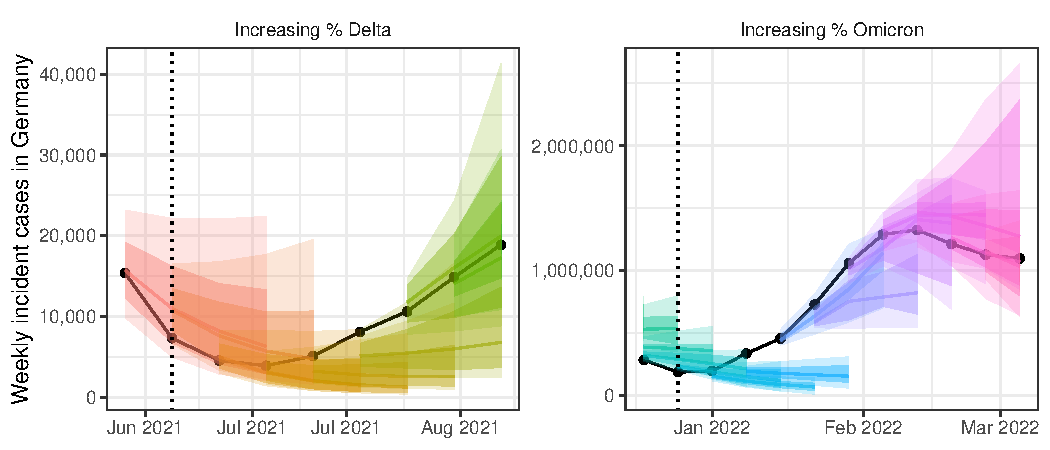
\includegraphics{abstract-results_files/figure-latex/figure-1-1.pdf}
\caption{\emph{Ensemble forecasts of weekly incident cases in Germany
over periods of increasing SARS-CoV-2 variants Delta (B.1.617.2, left)
and Omicron (B.1.1.529, right). Black indicates observed data. Coloured
ribbons represent each weekly forecast of 1-4 weeks ahead (showing
median, 50\%, and 90\% probability). For each variant, forecasts are
shown over an x-axis bounded by the earliest dates at which 5\% and 99\%
of sequenced cases were identified as the respective variant of concern,
while vertical dotted lines indicate the approximate date that the
variant reached dominance (\textgreater50\% sequenced cases).}}
\end{figure}

Using all models and the ensemble, we created 2106 forecasting scores
where each score summarises a unique combination of forecasting model,
variable, country, and week ahead horizon (SI figure 2). We
qualitatively reviewed the absolute performance of forecasts in terms of
accuracy in predicting numbers of incident cases and deaths. We observed
that forecasts were often most accurate in times of stable epidemic
behaviour, while struggling to accurately predict at longer horizons
around inflection points, for example during rapid changes in
population-level behaviour or surveillance. Forecast models varied
widely in their ability to predict and account for the introduction of
new variants, giving the ensemble forecast over these periods a high
level of uncertainty (figure 3). In this study we focus only on the
comparative performance of forecasting models relative to each other.

In relative terms, the ensemble of all models performed well compared to
both its component models and the baseline. By relative WIS scaled
against a baseline of 1 (where a score \textless1 indicates
outperforming the baseline), the median score for participating models
across all submitted forecasts was 1.04, while the median score of
forecasts from the ensemble model was 0.71.

Across all horizons and locations, the ensemble performed better on
scaled relative WIS than 84\% of participating model scores when
forecasting cases (with a total N=862), and 92\% of participating model
scores for forecasts of incident deaths (N=746).

\begin{figure}
\centering
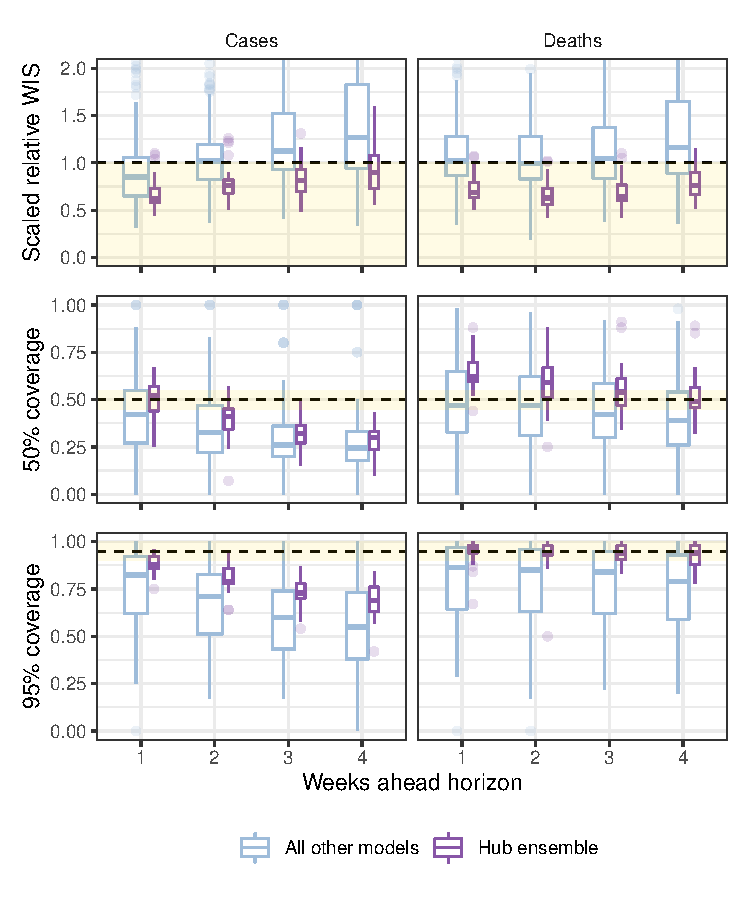
\includegraphics{abstract-results_files/figure-latex/figure-2-1.pdf}
\caption{\emph{Performance of short-term forecasts aggregated across all
individually submitted models and the Hub ensemble, by horizon,
forecasting cases (left) and deaths (right). Performance measured by
relative weighted interval score scaled against a baseline (dotted line,
1), and coverage of uncertainty at the 50\% and 95\% levels. Boxplot,
with width proportional to number of observations, show interquartile
ranges with outlying scores as faded points. The target range for each
set of scores is shaded in yellow.}}
\end{figure}

The performance of individual and ensemble forecasts varied by length of
the forecast horizon (figure 3). At each horizon, the typical
performance of the ensemble outperformed both the baseline model and the
aggregated scores of all its component models, although we saw wide
variation between individual models in performance across horizons.

Both individual models and the ensemble saw a trend of worsening
performance at longer horizons when forecasting cases, while performance
remained more stable when estimating deaths. By scaled relative WIS, the
median performance of the ensemble across locations worsened from 0.62
for one-week ahead forecasts to 0.9 when forecasting four weeks ahead.
Performance for forecasts of deaths was more stable over one through
four weeks, with median ensemble performance moving from 0.685 to 0.76
across the four week horizons.

We observed similar trends in performance across horizon when
considering how well the ensemble was calibrated with respect to the
observed data. At one week ahead the case ensemble was well calibrated
(ca. 50\% and 95\% nominal coverage at the 50\% and 95\% levels
respectively). This did not hold at longer forecast horizons as the case
forecasts became increasingly over-confident. Meanwhile, the ensemble of
death forecasts was well calibrated at the 95\% level across all
horizons, and the calibration of death forecasts at the 50\% level
increased in accuracy with lengthening horizons.

\begin{figure}
\centering
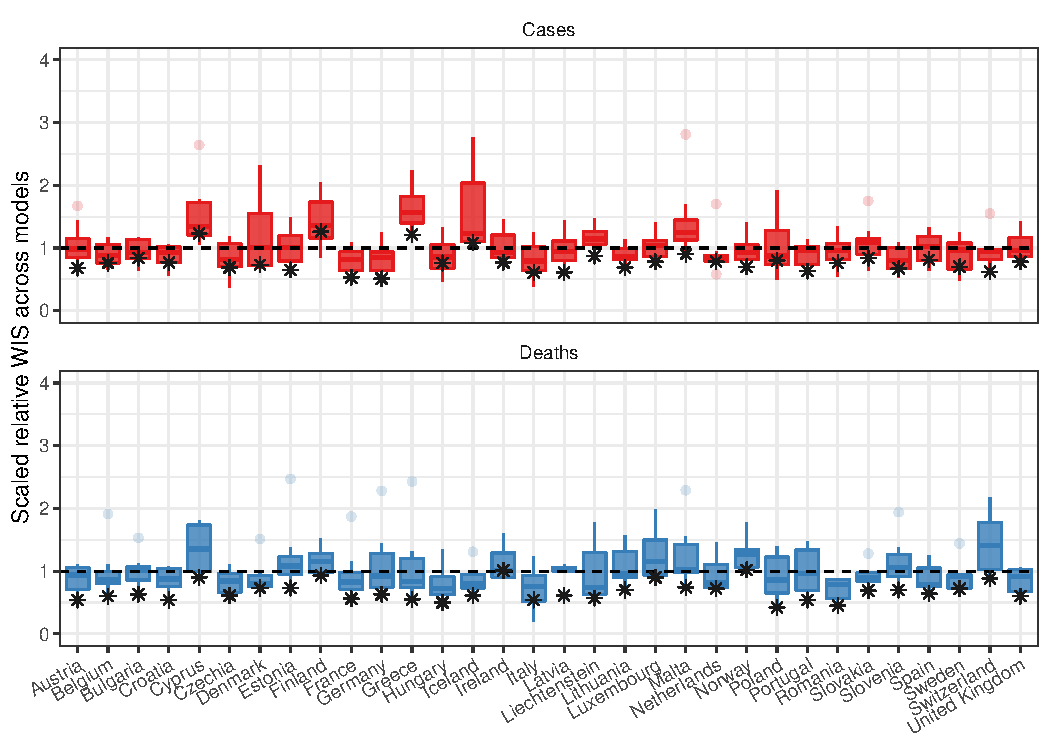
\includegraphics{abstract-results_files/figure-latex/figure-3-1.pdf}
\caption{\emph{Performance of short-term forecasts across models and
median ensemble (asterisk), by country, forecasting cases (top) and
deaths (bottom) for two-week ahead forecasts, according to the relative
weighted interval score. Boxplots show interquartile ranges, with
outliers as faded points, and the ensemble model performance is marked
by an asterisk. y-axis is cut-off to an upper bound of 4 for
readability.}}
\end{figure}

The ensemble also performed consistently well in comparison to
individual models when forecasting across countries (figure 3). Across
32 countries, on aggregate forecasting for one through four weeks, when
forecasting cases the ensemble oupterformed 75\% of component models in
21 countries, and outperformed all available models in 3 countries. When
forecasting deaths, the ensemble outperformed 75\% and 100\% of models
in 30 and 9 countries respectively. Considering only the the two-week
horizon shown in figure 3, the ensemble of case forecasts outperformed
75\% models in 24 countries and all models in only 12 countries. At the
two-week horizon for forecasts of deaths, the ensemble outperformed 75\%
and 100\% of its component models in 30 and 26 countries respectively.

\begin{table}

\caption{\label{tab:table-1}Predictive performance of main ensembles, as measured by the scaled relative WIS.}
\centering
\begin{tabular}[t]{lrrrr}
\toprule
Horizon & Weighted mean & Weighted median & Unweighted mean & Unweighted median\\
\midrule
\addlinespace[0.3em]
\multicolumn{5}{l}{\textbf{Cases}}\\
\hspace{1em}\cellcolor{gray!6}{1 week} & \cellcolor{gray!6}{0.59} & \cellcolor{gray!6}{0.62} & \cellcolor{gray!6}{0.59} & \cellcolor{gray!6}{0.61}\\
\hspace{1em}2 weeks & 0.67 & 0.67 & 0.67 & 0.67\\
\hspace{1em}\cellcolor{gray!6}{3 weeks} & \cellcolor{gray!6}{0.79} & \cellcolor{gray!6}{0.70} & \cellcolor{gray!6}{0.81} & \cellcolor{gray!6}{0.71}\\
\hspace{1em}4 weeks & 1.06 & 0.75 & 1.09 & 0.79\\
\addlinespace[0.3em]
\multicolumn{5}{l}{\textbf{Deaths}}\\
\hspace{1em}\cellcolor{gray!6}{1 week} & \cellcolor{gray!6}{0.63} & \cellcolor{gray!6}{0.59} & \cellcolor{gray!6}{1.00} & \cellcolor{gray!6}{0.59}\\
\hspace{1em}2 weeks & 0.57 & 0.54 & 0.81 & 0.53\\
\hspace{1em}\cellcolor{gray!6}{3 weeks} & \cellcolor{gray!6}{0.64} & \cellcolor{gray!6}{0.56} & \cellcolor{gray!6}{0.83} & \cellcolor{gray!6}{0.54}\\
\hspace{1em}4 weeks & 0.83 & 0.64 & 0.82 & 0.62\\
\bottomrule
\end{tabular}
\end{table}

We considered alternative methods for creating ensembles from the
participating forecasts, using either a mean or median to combine either
weighted or unweighted forecasts (table 1). Across locations we observed
that the median outperformed the mean across all one through four week
horizons and both cases and death targets, for all but cases at the 1
week horizon. This held regardless of whether the component forecasts
were weighted or unweighted by their individual past performance.
Between methods of combination, weighting made little difference to the
performance of the median ensemble, but slightly improved performance of
the mean ensemble.

\hypertarget{discussion}{%
\section{Discussion}\label{discussion}}

We collated 12 months of forecasts of COVID-19 cases and deaths across
32 countries in Europe, collecting from multiple independent teams and
using a principled approach to standardising both forecast targets and
the uncertainty around predictions. We combined these into an ensemble
forecast and compared the relative performance of forecasts among
models, finding that the ensemble forecasts produced among the most
consistent predictive performance across countries and horizons over
time compared to any individual model.

Our results support previous findings that ensemble forecasts are or are
near the best performing models with respect to error and appropriate
coverage of uncertainty
\protect\hyperlink{ref-funkShorttermForecastsInform2020}{{[}9{]}},
\protect\hyperlink{ref-cramerEvaluationIndividualEnsemble2021}{{[}28{]}},
\protect\hyperlink{ref-viboudRAPIDDEbolaForecasting2018}{{[}13{]}}.
While the ensemble was consistently high performing, it was not strictly
dominant across all forecast targets, with others also seeing this in
comparable studies of COVID-19 forecasts
\protect\hyperlink{ref-bracherPreregisteredShorttermForecasting2021}{{[}8{]}},
\protect\hyperlink{ref-brooksComparingEnsembleApproaches2020}{{[}34{]}}.
Our finding suggests the usefulness of an ensemble as a robust summary
when forecasting across many spatio-temporal targets, without replacing
the importance of communicating the full range of model predictions.

We identified the adaptability of an ensemble forecast to changing
conditions as a particular benefit from applying our approach to the
COVID-19 outbreak in Europe. As epidemic dynamics became increasingly
heterogeneous, the forecasting performance of any single model over time
and across multiple countries became at least partly dependent on the
ability, speed, and precision with which it could adapt to new
conditions for each forecast target. This variability in the relative
performance of models over time makes using an ensemble, balancing
across all models, particularly relevant in rapidly changing epidemic
conditions.

In particular, our results suggest the limited value of reporting case
forecasts further into the future. Previous work has similarly found
rapidly declining performance for case forecasts with increasing horizon
\protect\hyperlink{ref-cramerEvaluationIndividualEnsemble2021}{{[}28{]}},
\protect\hyperlink{ref-castroTurningPointEnd2020}{{[}35{]}}. COVID-19
has a typical serial interval of less than a week, which implies that
case forecasts of more than two weeks can only hold if rates of
transmission and detection remain predictable over the entire period. In
our study's context, this would be a strong assumption with many
instances of rapidly changing policies and individual behaviour observed
over the period.

In contrast, our results highlight the more stable performance of death
forecasts over lengthening time horizons. Specifically, we found the
ensemble in this study continued to outperform both other models and the
baseline at up to four weeks ahead. In general, previous work has found
death forecasts perform well with up to six weeks lead time
\protect\hyperlink{ref-friedmanPredictivePerformanceInternational2021}{{[}36{]}}.
We could interpret this as due to the longer time lag between infection
and death \protect\hyperlink{ref-jinLagDailyReported2021}{{[}37{]}}, and
higher consistency of reporting in surveillance data
\protect\hyperlink{ref-catalaRobustEstimationDiagnostic2021}{{[}38{]}},
which allow forecasters to incorporate the effect of changes in
transmission. Additionally, the performance of trend-based forecasts may
have benefited from the slower changes to trends in incident deaths
caused by increasing vaccination rates.

When exploring variations in ensemble methods, we found that the choice
of simple mean or median had the most consistent impact on performance,
regardless of the method of weighting. Other work has supported the
importance of the median in providing a stable forecast that better
accounts for outliers than the mean
\protect\hyperlink{ref-brooksComparingEnsembleApproaches2020}{{[}34{]}}.
However, our results did not show a strong performance benefit for any
one methodological choice, joining the existing mixed evidence for any
optimal ensemble method for combining short term probabilistic
infectious disease forecasts. In similar analyses of US COVID-19
forecasts many methods of combination have performed competitively,
including the simple mean and weighted approaches outperforming
unweighted or median methods
\protect\hyperlink{ref-taylorCombiningProbabilisticForecasts2021}{{[}30{]}}.
This contrasts with later analyses finding weighted methods to give
similar performance to a median average
\protect\hyperlink{ref-rayEnsembleForecastsCoronavirus2020e}{{[}7{]}},
\protect\hyperlink{ref-brooksComparingEnsembleApproaches2020}{{[}34{]}}.
We can partly explain this inconsistency if performance of each method
depends on the outcome being predicted (cases, deaths), its count
(incident, cumulative) and absolute level, the changing disease
dynamics, and the varying quality and quantity of forecasting teams over
time.

We also identified benefits of our approach beyond the results of this
analysis. Open access to visualised forecasts and data is useful for
both academics and the public in an emergency setting when forecasts can
influence individual to international actions that change epidemic
dynamics \protect\hyperlink{ref-basshuysenThreeWaysWhich2021}{{[}1{]}}.
Existing participatory modelling efforts for COVID-19 have been useful
for policy communication
\protect\hyperlink{ref-cdcCoronavirusDisease20192020}{{[}5{]}}, while
multi-country efforts have included only single models adapted to
country-specific parameters
\protect\hyperlink{ref-aguasModellingCOVID19Pandemic2020}{{[}39{]}},
\protect\hyperlink{ref-adibParticipatoryModellingApproach2021}{{[}40{]}},
\protect\hyperlink{ref-agostoMonitoringCOVID19Contagion2021}{{[}41{]}}.
By expanding participation to many modelling teams, our work can create
robust ensemble forecasts across Europe while allowing comparison across
forecasts built with different interpretations of current data, on a
like for like scale in real time. At the same time, collating
time-stamped predictions ensures that we can test true out-of-sample
performance of models and avoid retrospective claims of performance.
Testing the limits of forecasting ability with these comparisons forms
an important part of communicating any model-based prediction to
decision makers.

We noted several limitations in our approach to assessing the relative
performance of an ensemble among forecast models. Our results are the
outcome of evaluating forecasts against a specific performance metric
and baseline, where multiple options for evaluation exist and the choice
reflects the aim of the evaluation process. Here we have largely used
the weighted interval score
\protect\hyperlink{ref-gneitingStrictlyProperScoring2007}{{[}27{]}},
which attempts to balance the assessment of probabilistic forecast
sharpness with over- and under-prediction. Alternative metrics serve
different purposes. The log score would more strongly penalise a single
erroneous forecast and might be more useful for a very conservative
evaluation. Applying an equal level of tolerance to forecasts falling
within some range of the observed data, or using only the absolute error
of point forecasts, may be simpler metrics to communicate results to lay
audiences
\protect\hyperlink{ref-reichReplyBracherScoring2019}{{[}42{]}},
\protect\hyperlink{ref-bracherEvaluatingEpidemicForecasts2021}{{[}26{]}}.

We aimed to focus on comparing scores among the set of available models
rather than exploring absolute forecast accuracy relative to observed
data. To do this we applied a pairwise averaging method for the WIS,
which also meant that we created scores that were comparable between
models even when many forecasters contributed only partially across the
matrix of forecast targets. However, the pairwise method has not been
formally tested against simulated data and we have not independently
investigated its accuracy. We then normalised these scores against the
score of a flat-line forecast model for each target, but the choice of
appropriate baseline for epidemic forecast models is not clear. For
example, since epidemics are non-stationary and in theory follow an
exponential growth and decay, an alternative baseline could have
modelled a straight line on the log scale. The model used here is
supported by previous work
\protect\hyperlink{ref-cramerEvaluationIndividualEnsemble2021}{{[}28{]}},
and while previous evaluation in a similar context has suggested that
choice of baseline affects relative performance in general
\protect\hyperlink{ref-bracherNationalSubnationalShortterm2021}{{[}43{]}},
we believe this does not substantively affect the specific result that
ensembles outperform individual models. Further work could also consider
how well our results compare when using an alternative baseline suitable
for epidemics, for example an exponential growth model.

Our results could have been influenced by the sample of contributing
forecasts. We accepted all modelling teams' participation and teams used
a wide variety of methods, each with individual advantages and
limitations. Meanwhile, teams may have changed their forecast methods,
and entered and exited the hub over time. The ensemble therefore
included forecasts based on models with changing assumptions each week,
and we did not test how far the stability or methods of component
forecasts influenced the resulting ensemble. This could be significant,
for example during a time of low incidence, where including only
compartmental models in an ensemble improved predictive performance
relative to including forecasts from a wider variety of methods
\protect\hyperlink{ref-taylorCombiningProbabilisticForecasts2021}{{[}30{]}}.
However, the same study found the most consistent ensemble over time was
that which included all forecasts regardless of method, with performance
increasing with the number of forecast models, so our results are
unlikely to have changed by excluding any contributing forecasts.

Our assessment of forecast performance may have been inaccurate due to
limitations in the observed data against which we evaluated forecasts.
We sourced data from a globally aggregated database to maintain
compatibility across 32 countries
\protect\hyperlink{ref-dongInteractiveWebbasedDashboard2020}{{[}20{]}}.
However, this made it difficult to identify the origin of lags and
inconsistencies between national data streams, and to what extent these
could bias forecasts for different targets. In particular we saw some
real time data revised retrospectively, introducing bias in either
direction where the data used to create forecasts was not the same as
that used to evaluate it. We attempted to mitigate this using by using
an automated process for determining data revisions, and excluding
forecasts made at a time of missing, unreliable, or heavily revised
data.

We see additional scope to adapt the Hub format to the changing COVID-19
situation across Europe. We have extended the Forecast Hub
infrastructure to include short term forecasts for hospitalisations with
COVID-19, which is a challenging task due to limited data across the
locations covered by the hub. As the policy focus shifts from immediate
response to anticipating changes brought by vaccinations or the
geographic spread of new variants
\protect\hyperlink{ref-europeancentrefordiseasepreventionandcontrolOverviewImplementationCOVID192021}{{[}44{]}},
we are also separately investigating models for longer term scenarios in
addition to the short term forecasts in a similar framework to existing
scenario modelling work in the US
\protect\hyperlink{ref-borcheringModelingFutureCOVID192021}{{[}45{]}}.

This study raises many further questions which could inform epidemic
forecast modellers and users. The dataset created by the European
Forecast Hub is an openly accessible, standardised, and extensively
documented catalogue of real time forecasting work from a range of teams
and models across Europe
\protect\hyperlink{ref-europeancovid-19forecasthubEuropeanCovid19Forecast}{{[}22{]}},
and we recommend its use for further research on forecast performance.
In the code developed for this study we hope to provide a worked example
of downloading and using both the forecasts and their evaluation scores.

Most obviously, here we have identified the relative performance of an
ensemble approach compared to individual models without exploring the
absolute performance of forecasts in making accurate or useful
predictions. In retrospect, we both collected and created several
forecasts with substantial errors compared to observed data. Others have
observed persistent limitations on the ability to forecast infectious
disease outbreaks, due to the complexity of the system being modelled
\protect\hyperlink{ref-scarpinoPredictabilityInfectiousDisease2019}{{[}46{]}},
\protect\hyperlink{ref-castroTurningPointEnd2020}{{[}35{]}},
\protect\hyperlink{ref-rosenkrantzFundamentalLimitationsEfficiently2022}{{[}47{]}}
and models' sensitivity to both the basic and time-varying reproduction
numbers
\protect\hyperlink{ref-viboudRAPIDDEbolaForecasting2018}{{[}13{]}},
\protect\hyperlink{ref-coriKeyDataOutbreak2017}{{[}48{]}},
\protect\hyperlink{ref-desaiRealtimeEpidemicForecasting2019}{{[}49{]}}.

Over the study period, we saw multiple fundamental changes in viral-,
individual-, and population-level factors driving the transmission of
COVID-19 across Europe. In early 2021, the introduction of vaccination
started to change population-level associations between infections,
cases, and deaths
{[}\protect\hyperlink{ref-europeancentrefordiseasepreventionandcontrolInterimGuidanceBenefits2021}{{[}50{]}},
while the Delta variant emerged and became dominant in Europe
\protect\hyperlink{ref-europeancentrefordiseasepreventionandcontrolThreatAssessmentBrief2021}{{[}51{]}}.
Similarly from late 2021 we saw the interaction of individually waning
immunity during the emergence and global spread of the Omicron variant
\protect\hyperlink{ref-europeancentrefordiseasepreventionandcontrolAssessmentFurtherSpread2022}{{[}52{]}}.
Meanwhile, neither the extent nor timing of these factors were uniform
across European countries covered by the Forecast Hub
\protect\hyperlink{ref-europeancentrefordiseasepreventionandcontrolOverviewImplementationCOVID192021}{{[}44{]}}.
Future work could explore the impact on forecast models of changing
epidemiology at a broad spatial scale by combining analyses of trends
and turning points in cases and deaths with forecast performance, or
extending to include data on vaccination, variant, or policy changes
over time.

There is also a wide range of methods for combining forecasts which
could improve performance of an ensemble or continue to demonstrate the
value of a simple approach. This includes altering the inclusion
criteria of forecast models based on different thresholds of past
performance, excluding or including only forecasts that predict the
lowest- and highest-values (trimming)
\protect\hyperlink{ref-taylorCombiningProbabilisticForecasts2021}{{[}30{]}},
or using alternative weighting methods such as quantile regression
averaging
\protect\hyperlink{ref-funkShorttermForecastsInform2020}{{[}9{]}}.
Exploring these questions would add to our understanding of real time
performance, supporting and improving future forecasting efforts.

For applied public health work, we recommend adapting and using our
open-source infrastructure to standardise and improve epidemiological
forecasts. The hub structure maximises the transparency and accuracy of
real-time forecasts and can reduce reliance on individual models as a
basis for action during an epidemic. The benefits of combining multiple
models into an ensemble come from individual models' wide variation in
forecast performance across varying targets, and this is particularly
true during emerging epidemics where forecasters vary in how quickly
their models are able to adapt to new information. Setting up the
infrastructure for this could be an important component to future
epidemic and pandemic preparedness. As it is free to develop, highly
modular, and well documented, the infrastructure we have developed in
this project may make this easier and faster to do.

In conclusion, we have shown that during a rapidly evolving epidemic
spreading through multiple populations, an ensemble forecast performed
highly consistently across a large matrix of forecast targets, typically
outperforming the majority of its separate component models. In
addition, we have demonstrated some limits to predictability, especially
for case forecasts, while showing that ensemble methods based on past
model performance were unable to reliably improve forecast performance.
Our work constitutes a step towards both unifying COVID-19 forecasts and
improving our understanding of them.

\hypertarget{refs}{}
\begin{CSLReferences}{0}{0}
\leavevmode\vadjust pre{\hypertarget{ref-basshuysenThreeWaysWhich2021}{}}%
\CSLLeftMargin{{[}1{]} }
\CSLRightInline{P. van Basshuysen, L. White, D. Khosrowi, and M. Frisch,
{``Three {Ways} in {Which Pandemic Models May Perform} a {Pandemic},''}
\emph{Erasmus Journal for Philosophy and Economics}, vol. 14, no. 1, 1,
pp. 110-127-110-127, Jul. 2021, doi:
\href{https://doi.org/10.23941/ejpe.v14i1.582}{10.23941/ejpe.v14i1.582}.}

\leavevmode\vadjust pre{\hypertarget{ref-zelnerAccountingUncertaintyPandemic2021}{}}%
\CSLLeftMargin{{[}2{]} }
\CSLRightInline{J. Zelner, J. Riou, R. Etzioni, and A. Gelman,
{``Accounting for uncertainty during a pandemic,''} \emph{PATTER}, vol.
2, no. 8, Aug. 2021, doi:
\href{https://doi.org/10.1016/j.patter.2021.100310}{10.1016/j.patter.2021.100310}.}

\leavevmode\vadjust pre{\hypertarget{ref-jamesUseMisuseMathematical2021}{}}%
\CSLLeftMargin{{[}3{]} }
\CSLRightInline{L. P. James, J. A. Salomon, C. O. Buckee, and N. A.
Menzies, {``The {Use} and {Misuse} of {Mathematical Modeling} for
{Infectious Disease Policymaking}: {Lessons} for the {COVID-19
Pandemic},''} \emph{Med Decis Making}, vol. 41, no. 4, pp. 379--385, May
2021, doi:
\href{https://doi.org/10.1177/0272989X21990391}{10.1177/0272989X21990391}.}

\leavevmode\vadjust pre{\hypertarget{ref-reichCollaborativeMultiyearMultimodel2019}{}}%
\CSLLeftMargin{{[}4{]} }
\CSLRightInline{N. G. Reich \emph{et al.}, {``A collaborative multiyear,
multimodel assessment of seasonal influenza forecasting in the {United
States},''} \emph{PNAS}, vol. 116, no. 8, pp. 3146--3154, Feb. 2019,
doi:
\href{https://doi.org/10.1073/pnas.1812594116}{10.1073/pnas.1812594116}.}

\leavevmode\vadjust pre{\hypertarget{ref-cdcCoronavirusDisease20192020}{}}%
\CSLLeftMargin{{[}5{]} }
\CSLRightInline{CDC, {``Coronavirus {Disease} 2019 ({COVID-19}),''} Feb.
11, 2020.
\url{https://www.cdc.gov/coronavirus/2019-ncov/science/forecasting/forecasting.html}
(accessed Jan. 09, 2022).}

\leavevmode\vadjust pre{\hypertarget{ref-cramerUnitedStatesCOVID192021}{}}%
\CSLLeftMargin{{[}6{]} }
\CSLRightInline{E. Y. Cramer \emph{et al.}, {``The {United States
COVID-19 Forecast Hub} dataset,''} p. 2021.11.04.21265886, Nov. 2021,
doi:
\href{https://doi.org/10.1101/2021.11.04.21265886}{10.1101/2021.11.04.21265886}.}

\leavevmode\vadjust pre{\hypertarget{ref-rayEnsembleForecastsCoronavirus2020e}{}}%
\CSLLeftMargin{{[}7{]} }
\CSLRightInline{E. L. Ray \emph{et al.}, {``Ensemble {Forecasts} of
{Coronavirus Disease} 2019 ({COVID-19}) in the {U}.{S}.''} p.
2020.08.19.20177493, Aug. 2020, doi:
\href{https://doi.org/10.1101/2020.08.19.20177493}{10.1101/2020.08.19.20177493}.}

\leavevmode\vadjust pre{\hypertarget{ref-bracherPreregisteredShorttermForecasting2021}{}}%
\CSLLeftMargin{{[}8{]} }
\CSLRightInline{J. Bracher \emph{et al.}, {``A pre-registered short-term
forecasting study of {COVID-19} in {Germany} and {Poland} during the
second wave,''} \emph{Nat Commun}, vol. 12, no. 1, 1, p. 5173, Aug.
2021, doi:
\href{https://doi.org/10.1038/s41467-021-25207-0}{10.1038/s41467-021-25207-0}.}

\leavevmode\vadjust pre{\hypertarget{ref-funkShorttermForecastsInform2020}{}}%
\CSLLeftMargin{{[}9{]} }
\CSLRightInline{S. Funk \emph{et al.}, {``Short-term forecasts to inform
the response to the {Covid-19} epidemic in the {UK},''} \emph{medRxiv},
p. 2020.11.11.20220962, Nov. 2020, doi:
\href{https://doi.org/10.1101/2020.11.11.20220962}{10.1101/2020.11.11.20220962}.}

\leavevmode\vadjust pre{\hypertarget{ref-bicherSupportingCOVID19PolicyMaking2021}{}}%
\CSLLeftMargin{{[}10{]} }
\CSLRightInline{M. Bicher \emph{et al.}, {``Supporting {COVID-19
Policy-Making} with a {Predictive Epidemiological Multi-Model Warning
System},''} \emph{medRxiv}, p. 2020.10.18.20214767, Apr. 2021, doi:
\href{https://doi.org/10.1101/2020.10.18.20214767}{10.1101/2020.10.18.20214767}.}

\leavevmode\vadjust pre{\hypertarget{ref-reichAccuracyRealtimeMultimodel2019}{}}%
\CSLLeftMargin{{[}11{]} }
\CSLRightInline{N. G. Reich \emph{et al.}, {``Accuracy of real-time
multi-model ensemble forecasts for seasonal influenza in the {U}.{S},''}
\emph{PLoS Comput Biol}, vol. 15, no. 11, p. e1007486, Nov. 2019, doi:
\href{https://doi.org/10.1371/journal.pcbi.1007486}{10.1371/journal.pcbi.1007486}.}

\leavevmode\vadjust pre{\hypertarget{ref-johanssonOpenChallengeAdvance2019}{}}%
\CSLLeftMargin{{[}12{]} }
\CSLRightInline{M. A. Johansson \emph{et al.}, {``An open challenge to
advance probabilistic forecasting for dengue epidemics,''} \emph{PNAS},
vol. 116, no. 48, pp. 24268--24274, Nov. 2019, doi:
\href{https://doi.org/10.1073/pnas.1909865116}{10.1073/pnas.1909865116}.}

\leavevmode\vadjust pre{\hypertarget{ref-viboudRAPIDDEbolaForecasting2018}{}}%
\CSLLeftMargin{{[}13{]} }
\CSLRightInline{C. Viboud \emph{et al.}, {``The {RAPIDD} ebola
forecasting challenge: {Synthesis} and lessons learnt,''}
\emph{Epidemics}, vol. 22, pp. 13--21, Mar. 2018, doi:
\href{https://doi.org/10.1016/j.epidem.2017.08.002}{10.1016/j.epidem.2017.08.002}.}

\leavevmode\vadjust pre{\hypertarget{ref-buizzaIntroductionSpecialIssue2019}{}}%
\CSLLeftMargin{{[}14{]} }
\CSLRightInline{R. Buizza, {``Introduction to the special issue on {`25
years of ensemble forecasting'},''} \emph{Quarterly Journal of the Royal
Meteorological Society}, vol. 145, no. S1, pp. 1--11, 2019, doi:
\href{https://doi.org/10.1002/qj.3370}{10.1002/qj.3370}.}

\leavevmode\vadjust pre{\hypertarget{ref-moranEpidemicForecastingMessier2016}{}}%
\CSLLeftMargin{{[}15{]} }
\CSLRightInline{K. R. Moran \emph{et al.}, {``Epidemic {Forecasting} is
{Messier Than Weather Forecasting}: {The Role} of {Human Behavior} and
{Internet Data Streams} in {Epidemic Forecast},''} \emph{J Infect Dis},
vol. 214, pp. S404--S408, Dec. 2016, doi:
\href{https://doi.org/10.1093/infdis/jiw375}{10.1093/infdis/jiw375}.}

\leavevmode\vadjust pre{\hypertarget{ref-europeancovid-19forecasthubEuropeanCOVID19Forecast2021}{}}%
\CSLLeftMargin{{[}16{]} }
\CSLRightInline{European Covid-19 Forecast Hub, \emph{European {COVID-19
Forecast Hub}}. {covid19-forecast-hub-europe}, 2021.Available:
\url{https://github.com/covid19-forecast-hub-europe/covid19-forecast-hub-europe}}

\leavevmode\vadjust pre{\hypertarget{ref-cramerReichlabCovid19forecasthubRelease2021}{}}%
\CSLLeftMargin{{[}17{]} }
\CSLRightInline{E. Cramer \emph{et al.},
{``Reichlab/Covid19-forecast-hub: Release for {Zenodo}, 20210816,''}
Aug. 2021, doi:
\href{https://doi.org/10.5281/zenodo.5208210}{10.5281/zenodo.5208210}.}

\leavevmode\vadjust pre{\hypertarget{ref-wangReichlabCovidHubUtilsRepository2021}{}}%
\CSLLeftMargin{{[}18{]} }
\CSLRightInline{S. Y. Wang \emph{et al.}, {``Reichlab/{covidHubUtils}:
Repository release for {Zenodo},''} Aug. 2021, doi:
\href{https://doi.org/10.5281/zenodo.5207940}{10.5281/zenodo.5207940}.}

\leavevmode\vadjust pre{\hypertarget{ref-bracherGermanPolishCOVID192020}{}}%
\CSLLeftMargin{{[}19{]} }
\CSLRightInline{J. Bracher \emph{et al.}, \emph{The {German} and {Polish
COVID-19 Forecast Hub}}. 2020.Available:
\url{https://github.com/KITmetricslab/covid19-forecast-hub-de}}

\leavevmode\vadjust pre{\hypertarget{ref-dongInteractiveWebbasedDashboard2020}{}}%
\CSLLeftMargin{{[}20{]} }
\CSLRightInline{E. Dong, H. Du, and L. Gardner, {``An interactive
web-based dashboard to track {COVID-19} in real time,''} \emph{The
Lancet Infectious Diseases}, vol. 20, no. 5, pp. 533--534, May 2020,
doi:
\href{https://doi.org/10.1016/S1473-3099(20)30120-1}{10.1016/S1473-3099(20)30120-1}.}

\leavevmode\vadjust pre{\hypertarget{ref-europeancovid-19forecasthubCovid19forecasthubeuropeWiki}{}}%
\CSLLeftMargin{{[}21{]} }
\CSLRightInline{European Covid-19 Forecast Hub,
{``Covid19-forecast-hub-europe: {Wiki}.''}
\url{https://github.com/covid19-forecast-hub-europe/covid19-forecast-hub-europe}}

\leavevmode\vadjust pre{\hypertarget{ref-europeancovid-19forecasthubEuropeanCovid19Forecast}{}}%
\CSLLeftMargin{{[}22{]} }
\CSLRightInline{European Covid-19 Forecast Hub, {``European {Covid-19
Forecast Hub}.''} \url{https://covid19forecasthub.eu/index.html}}

\leavevmode\vadjust pre{\hypertarget{ref-epiforecastsProjectECDCEuropean2021}{}}%
\CSLLeftMargin{{[}23{]} }
\CSLRightInline{EpiForecasts, {``Project: {ECDC European COVID-19
Forecast Hub} - {Zoltar},''} 2021.
\url{https://www.zoltardata.com/project/238}}

\leavevmode\vadjust pre{\hypertarget{ref-reichZoltarForecastArchive2021}{}}%
\CSLLeftMargin{{[}24{]} }
\CSLRightInline{N. G. Reich, M. Cornell, E. L. Ray, K. House, and K. Le,
{``The {Zoltar} forecast archive, a tool to standardize and store
interdisciplinary prediction research,''} \emph{Sci Data}, vol. 8, no.
1, 1, p. 59, Feb. 2021, doi:
\href{https://doi.org/10.1038/s41597-021-00839-5}{10.1038/s41597-021-00839-5}.}

\leavevmode\vadjust pre{\hypertarget{ref-nikosibosseScoringutilsUtilitiesScoring2020}{}}%
\CSLLeftMargin{{[}25{]} }
\CSLRightInline{Nikos I Bosse, Sam Abbott, EpiForecasts, and Sebastian
Funk, \emph{Scoringutils: {Utilities} for {Scoring} and {Assessing
Predictions}}. 2020.Available:
\url{https://github.com/epiforecasts/scoringutils}}

\leavevmode\vadjust pre{\hypertarget{ref-bracherEvaluatingEpidemicForecasts2021}{}}%
\CSLLeftMargin{{[}26{]} }
\CSLRightInline{J. Bracher, E. L. Ray, T. Gneiting, and N. G. Reich,
{``Evaluating epidemic forecasts in an interval format,''} \emph{PLOS
Computational Biology}, vol. 17, no. 2, p. e1008618, Feb. 2021, doi:
\href{https://doi.org/10.1371/journal.pcbi.1008618}{10.1371/journal.pcbi.1008618}.}

\leavevmode\vadjust pre{\hypertarget{ref-gneitingStrictlyProperScoring2007}{}}%
\CSLLeftMargin{{[}27{]} }
\CSLRightInline{T. Gneiting and A. E. Raftery, {``Strictly {Proper
Scoring Rules}, {Prediction}, and {Estimation},''} \emph{Journal of the
American Statistical Association}, vol. 102, no. 477, pp. 359--378, Mar.
2007, doi:
\href{https://doi.org/10.1198/016214506000001437}{10.1198/016214506000001437}.}

\leavevmode\vadjust pre{\hypertarget{ref-cramerEvaluationIndividualEnsemble2021}{}}%
\CSLLeftMargin{{[}28{]} }
\CSLRightInline{E. Y. Cramer \emph{et al.}, {``Evaluation of individual
and ensemble probabilistic forecasts of {COVID-19} mortality in the
{US},''} \emph{medRxiv}, p. 2021.02.03.21250974, Jan. 2021, doi:
\href{https://doi.org/10.1101/2021.02.03.21250974}{10.1101/2021.02.03.21250974}.}

\leavevmode\vadjust pre{\hypertarget{ref-genestVincentizationRevisited1992}{}}%
\CSLLeftMargin{{[}29{]} }
\CSLRightInline{C. Genest, {``Vincentization {Revisited},''} \emph{The
Annals of Statistics}, vol. 20, no. 2, pp. 1137--1142, 1992,Available:
\url{https://www.jstor.org/stable/2242003}}

\leavevmode\vadjust pre{\hypertarget{ref-taylorCombiningProbabilisticForecasts2021}{}}%
\CSLLeftMargin{{[}30{]} }
\CSLRightInline{J. W. Taylor and K. S. Taylor, {``Combining
{Probabilistic Forecasts} of {COVID-19 Mortality} in the {United
States},''} \emph{Eur J Oper Res}, Jun. 2021, doi:
\href{https://doi.org/10.1016/j.ejor.2021.06.044}{10.1016/j.ejor.2021.06.044}.}

\leavevmode\vadjust pre{\hypertarget{ref-rayComparingTrainedUntrained2022}{}}%
\CSLLeftMargin{{[}31{]} }
\CSLRightInline{E. L. Ray \emph{et al.}, {``Comparing trained and
untrained probabilistic ensemble forecasts of {COVID-19} cases and
deaths in the {United States},''} Jan. 28, 2022. Accessed: Mar. 30,
2022. {[}Online{]}. Available: \url{http://arxiv.org/abs/2201.12387}}

\leavevmode\vadjust pre{\hypertarget{ref-harrellNewDistributionfreeQuantile1982}{}}%
\CSLLeftMargin{{[}32{]} }
\CSLRightInline{F. E. HARRELL and C. E. DAVIS, {``A new
distribution-free quantile estimator,''} \emph{Biometrika}, vol. 69, no.
3, pp. 635--640, Dec. 1982, doi:
\href{https://doi.org/10.1093/biomet/69.3.635}{10.1093/biomet/69.3.635}.}

\leavevmode\vadjust pre{\hypertarget{ref-rdocumentationCNORMVersionWeighted}{}}%
\CSLLeftMargin{{[}33{]} }
\CSLRightInline{RDocumentation, \emph{{cNORM} (version 2.0.3):
Weighted.quantile function}. Available:
\url{https://www.rdocumentation.org/packages/cNORM/versions/2.0.3/topics/weighted.quantile}}

\leavevmode\vadjust pre{\hypertarget{ref-brooksComparingEnsembleApproaches2020}{}}%
\CSLLeftMargin{{[}34{]} }
\CSLRightInline{L. Brooks, {``Comparing ensemble approaches for
short-term probabilistic {COVID-19} forecasts in the {U}.{S}.''} 2020.
\url{https://forecasters.org/blog/2020/10/28/comparing-ensemble-approaches-for-short-term-probabilistic-covid-19-forecasts-in-the-u-s/}
(accessed Jul. 15, 2021).}

\leavevmode\vadjust pre{\hypertarget{ref-castroTurningPointEnd2020}{}}%
\CSLLeftMargin{{[}35{]} }
\CSLRightInline{M. Castro, S. Ares, J. A. Cuesta, and S. Manrubia,
{``The turning point and end of an expanding epidemic cannot be
precisely forecast,''} \emph{Proceedings of the National Academy of
Sciences}, vol. 117, no. 42, pp. 26190--26196, Oct. 2020, doi:
\href{https://doi.org/10.1073/pnas.2007868117}{10.1073/pnas.2007868117}.}

\leavevmode\vadjust pre{\hypertarget{ref-friedmanPredictivePerformanceInternational2021}{}}%
\CSLLeftMargin{{[}36{]} }
\CSLRightInline{J. Friedman \emph{et al.}, {``Predictive performance of
international {COVID-19} mortality forecasting models,''} \emph{Nat
Commun}, vol. 12, no. 1, 1, p. 2609, May 2021, doi:
\href{https://doi.org/10.1038/s41467-021-22457-w}{10.1038/s41467-021-22457-w}.}

\leavevmode\vadjust pre{\hypertarget{ref-jinLagDailyReported2021}{}}%
\CSLLeftMargin{{[}37{]} }
\CSLRightInline{R. Jin, {``The lag between daily reported {Covid-19}
cases and deaths and its relationship to age,''} \emph{J Public Health
Res}, vol. 10, no. 3, p. 2049, Mar. 2021, doi:
\href{https://doi.org/10.4081/jphr.2021.2049}{10.4081/jphr.2021.2049}.}

\leavevmode\vadjust pre{\hypertarget{ref-catalaRobustEstimationDiagnostic2021}{}}%
\CSLLeftMargin{{[}38{]} }
\CSLRightInline{M. Català \emph{et al.}, {``Robust estimation of
diagnostic rate and real incidence of {COVID-19} for {European}
policymakers,''} \emph{PLOS ONE}, vol. 16, no. 1, p. e0243701, Jan.
2021, doi:
\href{https://doi.org/10.1371/journal.pone.0243701}{10.1371/journal.pone.0243701}.}

\leavevmode\vadjust pre{\hypertarget{ref-aguasModellingCOVID19Pandemic2020}{}}%
\CSLLeftMargin{{[}39{]} }
\CSLRightInline{R. Aguas \emph{et al.}, {``Modelling the {COVID-19}
pandemic in context: An international participatory approach,''}
\emph{BMJ Global Health}, vol. 5, no. 12, p. e003126, Dec. 2020, doi:
\href{https://doi.org/10.1136/bmjgh-2020-003126}{10.1136/bmjgh-2020-003126}.}

\leavevmode\vadjust pre{\hypertarget{ref-adibParticipatoryModellingApproach2021}{}}%
\CSLLeftMargin{{[}40{]} }
\CSLRightInline{K. Adib \emph{et al.}, {``A participatory modelling
approach for investigating the spread of {COVID-19} in countries of the
{Eastern Mediterranean Region} to support public health
decision-making,''} \emph{BMJ Global Health}, vol. 6, no. 3, p. e005207,
Mar. 2021, doi:
\href{https://doi.org/10.1136/bmjgh-2021-005207}{10.1136/bmjgh-2021-005207}.}

\leavevmode\vadjust pre{\hypertarget{ref-agostoMonitoringCOVID19Contagion2021}{}}%
\CSLLeftMargin{{[}41{]} }
\CSLRightInline{A. Agosto, A. Campmas, P. Giudici, and A. Renda,
{``Monitoring {COVID-19} contagion growth,''} \emph{Statistics in
Medicine}, vol. 40, no. 18, pp. 4150--4160, 2021, doi:
\href{https://doi.org/10.1002/sim.9020}{10.1002/sim.9020}.}

\leavevmode\vadjust pre{\hypertarget{ref-reichReplyBracherScoring2019}{}}%
\CSLLeftMargin{{[}42{]} }
\CSLRightInline{N. G. Reich \emph{et al.}, {``Reply to {Bracher}:
{Scoring} probabilistic forecasts to maximize public health
interpretability,''} \emph{Proceedings of the National Academy of
Sciences}, vol. 116, no. 42, pp. 20811--20812, Oct. 2019, doi:
\href{https://doi.org/10.1073/pnas.1912694116}{10.1073/pnas.1912694116}.}

\leavevmode\vadjust pre{\hypertarget{ref-bracherNationalSubnationalShortterm2021}{}}%
\CSLLeftMargin{{[}43{]} }
\CSLRightInline{J. Bracher \emph{et al.}, {``National and subnational
short-term forecasting of {COVID-19} in {Germany} and {Poland}, early
2021,''} p. 2021.11.05.21265810, Nov. 2021, doi:
\href{https://doi.org/10.1101/2021.11.05.21265810}{10.1101/2021.11.05.21265810}.}

\leavevmode\vadjust pre{\hypertarget{ref-europeancentrefordiseasepreventionandcontrolOverviewImplementationCOVID192021}{}}%
\CSLLeftMargin{{[}44{]} }
\CSLRightInline{European Centre for Disease Prevention and Control,
{``Overview of the implementation of {COVID-19} vaccination strategies
and deployment plans in the {EU}/{EEA},''} {ECDC}, {Stockholm}, Nov.
2021.Available:
\url{https://www.ecdc.europa.eu/en/publications-data/overview-implementation-covid-19-vaccination-strategies-and-deployment-plans}}

\leavevmode\vadjust pre{\hypertarget{ref-borcheringModelingFutureCOVID192021}{}}%
\CSLLeftMargin{{[}45{]} }
\CSLRightInline{R. K. Borchering, {``Modeling of {Future COVID-19
Cases}, {Hospitalizations}, and {Deaths}, by {Vaccination Rates} and
{Nonpharmaceutical Intervention Scenarios} --- {United States},
{April}--{September} 2021,''} \emph{MMWR Morb Mortal Wkly Rep}, vol. 70,
2021, doi:
\href{https://doi.org/10.15585/mmwr.mm7019e3}{10.15585/mmwr.mm7019e3}.}

\leavevmode\vadjust pre{\hypertarget{ref-scarpinoPredictabilityInfectiousDisease2019}{}}%
\CSLLeftMargin{{[}46{]} }
\CSLRightInline{S. V. Scarpino and G. Petri, {``On the predictability of
infectious disease outbreaks,''} \emph{Nat Commun}, vol. 10, no. 1, 1,
p. 898, Feb. 2019, doi:
\href{https://doi.org/10.1038/s41467-019-08616-0}{10.1038/s41467-019-08616-0}.}

\leavevmode\vadjust pre{\hypertarget{ref-rosenkrantzFundamentalLimitationsEfficiently2022}{}}%
\CSLLeftMargin{{[}47{]} }
\CSLRightInline{D. J. Rosenkrantz \emph{et al.}, {``Fundamental
limitations on efficiently forecasting certain epidemic measures in
network models,''} \emph{Proceedings of the National Academy of
Sciences}, vol. 119, no. 4, p. e2109228119, Jan. 2022, doi:
\href{https://doi.org/10.1073/pnas.2109228119}{10.1073/pnas.2109228119}.}

\leavevmode\vadjust pre{\hypertarget{ref-coriKeyDataOutbreak2017}{}}%
\CSLLeftMargin{{[}48{]} }
\CSLRightInline{A. Cori \emph{et al.}, {``Key data for outbreak
evaluation: Building on the {Ebola} experience,''} \emph{Philosophical
Transactions of the Royal Society B: Biological Sciences}, vol. 372, no.
1721, p. 20160371, May 2017, doi:
\href{https://doi.org/10.1098/rstb.2016.0371}{10.1098/rstb.2016.0371}.}

\leavevmode\vadjust pre{\hypertarget{ref-desaiRealtimeEpidemicForecasting2019}{}}%
\CSLLeftMargin{{[}49{]} }
\CSLRightInline{A. N. Desai \emph{et al.}, {``Real-time {Epidemic
Forecasting}: {Challenges} and {Opportunities},''} \emph{Health Secur},
vol. 17, no. 4, pp. 268--275, 2019 Jul/Aug, doi:
\href{https://doi.org/10.1089/hs.2019.0022}{10.1089/hs.2019.0022}.}

\leavevmode\vadjust pre{\hypertarget{ref-europeancentrefordiseasepreventionandcontrolInterimGuidanceBenefits2021}{}}%
\CSLLeftMargin{{[}50{]} }
\CSLRightInline{European Centre for Disease Prevention and Control,
{``Interim guidance on the benefits of full vaccination against
{COVID-19} for transmission and implications for non-pharmaceutical
interventions - 21 {April} 2021,''} {ECDC}, {Stockholm}, 2021.Available:
\url{https://www.ecdc.europa.eu/en/publications-data/interim-guidance-benefits-full-vaccination-against-covid-19-transmission}}

\leavevmode\vadjust pre{\hypertarget{ref-europeancentrefordiseasepreventionandcontrolThreatAssessmentBrief2021}{}}%
\CSLLeftMargin{{[}51{]} }
\CSLRightInline{European Centre for Disease Prevention and Control,
{``Threat {Assessment Brief}: {Implications} for the {EU}/{EEA} on the
spread of the {SARS-CoV-2 Delta} ({B}.1.617.2) variant of concern,''}
{ECDC}, {Stockholm}, Jun. 2021.Available:
\url{https://www.ecdc.europa.eu/en/publications-data/threat-assessment-emergence-and-impact-sars-cov-2-delta-variant}}

\leavevmode\vadjust pre{\hypertarget{ref-europeancentrefordiseasepreventionandcontrolAssessmentFurtherSpread2022}{}}%
\CSLLeftMargin{{[}52{]} }
\CSLRightInline{European Centre for Disease Prevention and Control,
{``Assessment of the further spread and potential impact of the
{SARS-CoV-2 Omicron} variant of concern in the {EU}/{EEA}, 19th
update,''} Jan. 27, 2022.
\url{https://www.ecdc.europa.eu/en/publications-data/covid-19-omicron-risk-assessment-further-emergence-and-potential-impact}}

\end{CSLReferences}

\end{document}
